%% abtex2-modelo-projeto-pesquisa.tex, v<VERSION> laurocesar
%% Copyright 2012-<COPYRIGHT_YEAR> by abnTeX2 group at http://www.abntex.net.br/
%%
%% This work may be distributed and/or modified under the
%% conditions of the LaTeX Project Public License, either version 1.3
%% of this license or (at your option) any later version.
%% The latest version of this license is in
%%   http://www.latex-project.org/lppl.txt
%% and version 1.3 or later is part of all distributions of LaTeX
%% version 2005/12/01 or later.
%%
%% This work has the LPPL maintenance status `maintained'.
%%
%% The Current Maintainer of this work is the abnTeX2 team, led
%% by Lauro César Araujo. Further information are available on
%% http://www.abntex.net.br/
%%
%% This work consists of the files abntex2-modelo-projeto-pesquisa.tex
%% and abntex2-modelo-references.bib
%%

% ------------------------------------------------------------------------
% ------------------------------------------------------------------------
% abnTeX2: Modelo de Projeto de pesquisa em conformidade com
% ABNT NBR 15287:2011 Informação e documentação - Projeto de pesquisa -
% Apresentação
% ------------------------------------------------------------------------
% ------------------------------------------------------------------------

\documentclass[
	% -- opções da classe memoir --
	12pt,				% tamanho da fonte
	%openright,			% capítulos começam em pág ímpar (insere página vazia caso preciso)
	oneside,			% para impressão em recto e verso. Oposto a oneside
	a4paper,			% tamanho do papel.
	% -- opções da classe abntex2 --
	%chapter=TITLE,		% títulos de capítulos convertidos em letras maiúsculas
	%section=TITLE,		% títulos de seções convertidos em letras maiúsculas
	%subsection=TITLE,	% títulos de subseções convertidos em letras maiúsculas
	%subsubsection=TITLE,% títulos de subsubseções convertidos em letras maiúsculas
	% -- opções do pacote babel --
	brazil,			    % idioma adicional para hifenização
	french,				% idioma adicional para hifenização
	spanish,			% idioma adicional para hifenização
	english,			% o último idioma é o principal do documento
	]{abntex2}

% ---
% PACOTES
% ---

% ---
% Pacotes fundamentais
% ---
\usepackage{lmodern}			% Usa a fonte Latin Modern
\usepackage[T1]{fontenc}		% Selecao de codigos de fonte.
\usepackage[utf8]{inputenc}		% Codificacao do documento (conversão automática dos acentos)
\usepackage{indentfirst}		% Indenta o primeiro parágrafo de cada seção.
\usepackage{color}				% Controle das cores
\usepackage{graphicx}			% Inclusão de gráficos
\usepackage{microtype} 			% para melhorias de justificação
% ---

% ---
% Pacotes adicionais
% ---
\usepackage{pdflscape}
\usepackage{adjustbox}
\usepackage{capa-epusp-abntex2}
\usepackage{pgfgantt} % gantt plot
\usepackage{rotating}
\usepackage[graphicx]{realboxes}
\usepackage[babel=true, kerning=true]{microtype} % required for gantt plot work
\usepackage{csquotes} % for babel
% ---

% ---
% Pacotes de citações
% ---
\usepackage[
    style=abnt,
    %style=authoryear,
    %citestyle=authoryear,
    %bibstyle=authortitle,
    %sorting=ynt,
    %backend=bibtex,
    %clearlang=true,
    %language=english,
    %natbib=true,
    %maxbibnames=99,
    %noslsn=true,
    %firstinits=true,
    %block=ragged,
    %ittitles,
    ]{biblatex}	% Citações padrão ABNT
\addbibresource{biblio_biblatex.bib}

% ---
% Informações de dados para CAPA e FOLHA DE ROSTO
% ---
\titulo{Identification of sugarcane weeds by neural networks in FPGAs}
\autor{Vitor Finotti Ferreira}
\local{São Paulo}
\data{2017}
\instituicao{%
  Universidade de São Paulo
  \par
  Escola Politécnica
  \par
  Programa de Pós-Graduação - Engenharia de Computação e Sistemas Digitais}
\tipotrabalho{Master of Science Thesis}
\areaconcentracao{Computational Engineering}
% O preambulo deve conter o tipo do trabalho, o objetivo,
% o nome da instituição e a área de concentração
\preambulo{Proposal of a master thesis on the implementation of neural networks on Field Programmable Gate Arrays for identification of sugarcane weeds.}
% ---

% ---
% Configurações de aparência do PDF final

% alterando o aspecto da cor azul
\definecolor{blue}{RGB}{41,5,195}

% informações do PDF
\makeatletter
\hypersetup{
     	%pagebackref=true,
		pdftitle={\@title},
		pdfauthor={\@author},
    	pdfsubject={\imprimirpreambulo},
	    pdfcreator={LaTeX with abnTeX2},
		pdfkeywords={abnt}{latex}{abntex}{abntex2}{projeto de pesquisa},
		colorlinks=true,       		% false: boxed links; true: colored links
    	linkcolor=blue,          	% color of internal links
    	citecolor=blue,        		% color of links to bibliography
    	filecolor=magenta,      		% color of file links
		urlcolor=blue,
		bookmarksdepth=4
}
\makeatother
% ---

% ---
% Espaçamentos entre linhas e parágrafos
% ---

% O tamanho do parágrafo é dado por:
\setlength{\parindent}{1.3cm}

% Controle do espaçamento entre um parágrafo e outro:
\setlength{\parskip}{0.2cm}  % tente também \onelineskip

% ---
% compila o indice
% ---
\makeindex
% ---

% ---
% Configurações do Gráfico de Gantt
% ---
\newganttchartelement*{mymilestone}{
mymilestone/.style={
shape=isosceles triangle,
inner sep=0pt,
draw=cyan,
top color=white,
bottom color=cyan!50
},
mymilestone incomplete/.style={
/pgfgantt/mymilestone,
draw=yellow,
bottom color=yellow!50
},
mymilestone label font=\slshape,
mymilestone left shift=0pt,
mymilestone right shift=0pt
}

\newgantttimeslotformat{stardate}{%
\def\decomposestardate##1.##2\relax{%
\def\stardateyear{##1}\def\stardateday{##2}%
}%
\decomposestardate#1\relax%
\pgfcalendardatetojulian{\stardateyear-01-01}{#2}%
\advance#2 by-1\relax%
\advance#2 by\stardateday\relax%
}

% ----
% Início do documento
% ----
\begin{document}

% Seleciona o idioma do documento (conforme pacotes do babel)
\selectlanguage{english}
%\selectlanguage{brazil}

% Retira espaço extra obsoleto entre as frases.
\frenchspacing

% ----------------------------------------------------------
% ELEMENTOS PRÉ-TEXTUAIS
% ----------------------------------------------------------
% \pretextual

% ---
% Capa
% ---
\imprimircapa
% ---

% ---
% Folha de rosto
% ---
\imprimirfolhaderosto
% ---

% ---
% NOTA DA ABNT NBR 15287:2011, p. 4:
%  ``Se exigido pela entidade, apresentar os dados curriculares do autor em
%     folha ou página distinta após a folha de rosto.''
% ---

% ---
% RESUMOS
% ---

% resumo em inglês
\begin{resumo}
  The sugarcane cultivation has a prominent role in the Brazilian agribusiness, being used not only in the food sector but also as an energy resource. In situations where the cultivation focus is the growth and production of organic products, limitations on pesticides and agrochemicals usage leads to the urge to find alternatives to control pests such as the \textit{Ipomoea grandifolia}, a weed that affect sugarcane plantation. This work proposes to implement a neural network in FPGA capable of identifying this weed, working as a first stage of a system to combat it.

   \vspace{\onelineskip}
 
   \noindent 
   \textbf{Keywords}: Sugarcane, FPGA, Neural Networks.
\end{resumo}


% resumo em português
\setlength{\absparsep}{18pt} % ajusta o espaçamento dos parágrafos do resumo
\begin{resumo}[Resumo]
\begin{otherlanguage*}{brazil}
 O cultivo de cana-de-açúcar tem um papel de destaque dentro do agronegócio brasileiro, tendo participação tanto como matéria prima alimentícia quanto energética. Quando o foco do cultivo é a produção de produtos orgânicos, limitações quanto aos pesticidas e agrotóxicos usados geram uma necessidade de encontrar alternativas para controlar pragas tais como o cipó \textit{Ipomoea grandifolia}. Este trabalho propõe implementar uma rede neural em FPGA capaz de identificar esta planta daninha por imagem, de forma a ser a primeira etapa em um sistema de combate a ela.

 \textbf{Palavras-chave}: Cana-de-açúcar, FPGA, Redes Neurais.
  \end{otherlanguage*}
\end{resumo}


% ---
% inserir o sumario
% ---
\pdfbookmark[0]{\contentsname}{toc}
\tableofcontents*
\cleardoublepage
% ---


% ----------------------------------------------------------
% ELEMENTOS TEXTUAIS
% ----------------------------------------------------------
\textual

% ----------------------------------------------------------
% Introdução
% ----------------------------------------------------------

\chapter[Introduction \& Background]{Introduction \& Background}
%Introduce the area of research 
%Review key publications
%Identify any gap in the knowledge or questions which have to be answered
%Your hypotheses
%Your aims and objectives, including a brief description of the methodology
%How is your research beneficial and to whom
  
  The agribusiness has a major importance in the Brazilian economy, promoting not only agriculture and cattle raising, but also the technological and logistical infrastructure that supports the sectors. This encompasses several areas related to agriculture, both upstream and downstream, involving: production of inputs for agriculture, production of agricultural raw materials, processing of these raw materials, distribution and other services, up to final consumption or export.~\cite{cepea}. In 2016, agribusiness accounted for 23\% of national GDP, moving R\$ 1.425 trillion~\cite{cna}, being a fundamental mitigating factor in the economic crisis that the country experienced~\cite{agro_canal_rural}.
  
  Among the various activities that make up agribusiness, sugarcane cultivation plays an important role, with its production chain accounting for R\$ 164.181 billions in 2016 \cite{cna}. Amid the needs of sugarcane production there is a niche focused on organic products, whose production is characterised by social, environmental and economic sustainability~\cite{organicos_canal_rural}. Among its particularities there is the non-use of agrochemicals, hormones, veterinary drugs, chemical fertilisers, antibiotics or transgenic products at any stage of production. The benefits gained by these restrictions contrast with the difficulty in increasing the scale of production and maintaining the competitive cost, which concentrates this market in small producers, limiting the access of their benefits to the population. Although with great potential, the market for organic products is still characterised by a timid supply compared to the growing demand~\cite{organicos_carta_capital}.
  
  The development of technologies that can support the growth of this sector are fundamental to develop their national potential, whose market share is 10 times lower than traditional markets, such as the US or Germany~\cite{organicos_carta_capital}.
  
% Ligar com o texto dos objetivos explicando como é feito o controle atualmente em lavouras organicas.
% Hoje, o produtor contrata um ser humano pra ir de tempos em tempos lá e cortar manualmente. O que acontece é que a lavoura de cana de acucar é agressiva para o ser humano, oferencendo riscos como cortes, fogo, animais peconhentos, etc. A ideia final é identificar remotamente os cipos para que o corte possa ser feito somente quando necessario, preferencialmente por um equipamento autonomo.
% Nas lavouras organicas nao pode-se entrar com maquinario pesado pois o solo é "vivo", com uma microfauna importante para manutençao da lavoura. As maquinas pesadas danificam este ambiente e são consideradas inadequadas para o cultivo organico. Todo maquinario, emsmo leve, é preparado para não compactar o solo.
% Robos agricolas não sao adequados para supervisao remota pois dependem de bateria e a comunicacao é precaria por causa da presenca de agua (nas canas de acucar).

%  O controle de pragas nestas plantações organicas é feito através do uso de mão de obra humana, onde um trabalhador contratado percorre a plantação periodicamente para lidar com elas manualmente. No caso do cipó textit{Ipomoea grandifolia}, erva daninha que atinge a cana-de-açúcar, o trabalhador procura uma flor branca característica do cipó, cortando-a ao encontrar. Contudo, tais ambientes de plantação são agressivos ao ser humano, oferecendo riscos como animais peçonhentos, cortes e fogo. A ideia deste projeto é identificar o cipó remotamente para que as intervenções na plantação sejam feitas apenas quando necessário, de preferência por um equipamento autônomo.

  Pest control in these organic plantations is done through the use of human labour, where a hired worker periodically traverses the plantation to deal with them manually. In the case of the \textit{Ipomoea grandifolia}, a weed that affects sugarcane, the worker searches for a flower characteristic of the vine, illustrated on \autoref{fig:ipomoea}, cutting it when found. However, such planting environments are aggressive to humans, posing hazards such as venomous animals, cuts and fire. The idea of this project is to identify the vine remotely so that the interventions in the plantation are made only when necessary, preferably by an autonomous equipment.
  
  \begin{figure}[htb]
	\caption{\label{fig:ipomoea}\textit{Ipomoea grandifolia} vine}
	\begin{center}
	    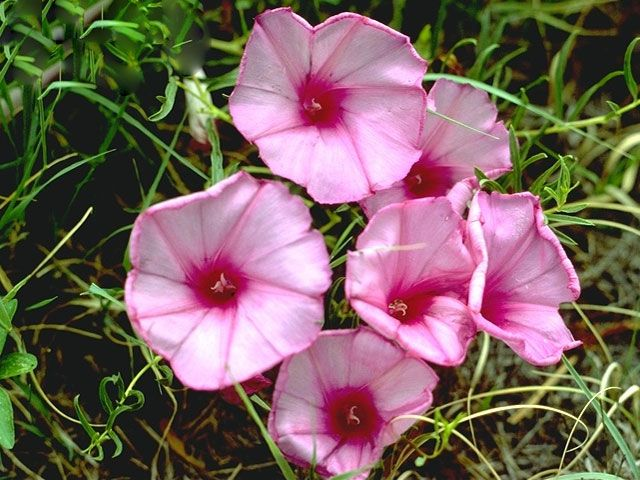
\includegraphics[scale=0.5]{images/Ipomoea_grandifolia76.jpg}
	\end{center}
	\legend{Source: \cite{corda_viola_agrolink}}
\end{figure}

  
%  Nas lavouras orgânicas a utilização de maquinário pesado também não é possível, pois a utilização destes afetam uma microfauna presente no solo que é importante para a manutenção da lavoura. Máquinas pesadas danificam este ambiente e são inadequadas para o cultivo orgânico. Todo maquinário, mesmo leve, é preparado para não compactar o solo. Neste contexto, robôs agrícolas não são adequados para supervisão remota por dependerem de uma bateria, cuja autonomia é limitada, e pela comunicação precária entre robô e central de processamento por conta da presença de água (da cana de açucar) no meio.
  
  In organic farming the use of heavy machinery is also not possible as it affects a micro fauna present in the soil, which is important for the maintenance of the crop. Heavy machinery damages this environment and is unsuitable for organic farming. All machinery, even light one, is prepared not to compact the soil. In this context, agricultural robots are not suitable for remote supervision because they depend on a battery, whose autonomy is limited, and the poor communication between robot and processing centre due to the presence of water (of sugarcane) in the medium.
  
  This project proposes to implement a convolutional neural network in an FPGA in order to perform the image recognition of the \textit{Ipomoea grandifolia} vine, seeking to provide an effective and energy efficient solution for the problem.
  
    
\chapter[Objectives]{Objectives}
 
 This work aims to implement a convolutional neural network in FPGA capable of identifying the \textit{Ipomoea grandifolia}, a weed that affects sugarcane. Such identification would be the first stage of a system for the control of this pest. The FPGA implementation is attractive due its high parallelization capacity and the reduced power consumption compared to other hardware architectures such as GPUs. These characteristics are important in the context of a rural plantation where poor internet access requires that the processing be done  autonomously on the local, and the limited access to energy and demands a power efficient solution.
 
 

\chapter[Methodology]{Methodology}
\section{Investigation Approach}

Considering the popularity and effectiveness of convolutional neural networks on the field of image recognition~\cite{LeCun2015}, the project intends to implement such algorithm for the vine identification, using optimizations such as binary neural networks to improve hardware performance and efficiency~\cite{Nurvitadhi2017_0, Courbariaux2015}. Although other architectures like CPU and GPU offer high peak theoretical performance, the nature of binary neural network makes its implementation on customizable hardware more efficient. In this scenario, FPGAs provide orders of magnitude over software without having to use a fixed solution, such as ASICs~\cite{Courbariaux2015}.

The first step towards the implementation is the study of the theory and background of neural network and image recognition for hardware accelerators. This will be done choosing appropriate disciplines simultaneously with the literature review so the most recent advances on the field can guide the theoretical development, as planned on \autoref{sec:scheadule}.

The knowledge obtained will be applied to develop the structure of a binary convolutional neural network to do the image recognition task. Recent studies, such as \textcite{Nurvitadhi2017_0} shows the potential of FPGAs in comparison with other architectures in terms of energy efficiency. This potential is explored through specific optimizations on the neural network architecture, as mentioned on \textcites{Courbariaux2015, Zhang2017}. A training and test set of images of the \textit{Ipomoea grandifolia}, probably obtained from an organic sugarcane production farm, will be used to train the network and test its effectiveness in recognising the vine. This network will be trained using open-source tools.

Once the neural network is fully trained and tested, the implementation on hardware will begin. Tests to compare the performance and power consumption of the neural network on different architectures will be done, focusing in improving the energy efficiency. The implemented network will be validated through simulations and empirical tests, using real or emulated data.

Some studies show that FPGAs could outperform GPUs on next generations, using the combinations of numerous improvements made on FPGA together with DNN algorithm innovations that favour hardware customizability \cite{Nurvitadhi2017_1}. Achieving this performance on the FPGA could benefit not only this study, but also other applications that require not only energy efficience, but also high performance. Therefore, an effort will be made to improve the performance of the binary neural network as well.

\section{Tools and Resources}

  It is proposed to develop the project using open-source tools to reduce the cost of implementation and assist the dissemination of the technology created whenever possible. For the development phase, it will be used a computer with Linux operating system and software development environments such as Python and R. Since it is often necessary to use specific programs of the FPGA manufacturer for FPGA simulation, syntheses and implementation, private software such as Vivado or Quartus will be used. The infrastructure of the laboratories of the university will be used for the development and validation of the work done. Data for test and validation will be obtained from the an organic sugarcane production farm.

        
\section{Schedule} \label{sec:scheadule}
\begin{enumerate}
	\item Discipline 1; %item 1
	\item Discipline 2; %item 2
	\item Discipline 3; %item 3
	\item Discipline 4; %item 4
	\item Discipline 5; %item 5
	\item Literature Review; %item 6
	\item Application Analysis; %item 7
	\item System Implementation; %item 8
	\item System Validation; %item 9
	\item Qualification Exam; %item 10
	\item Thesis Writing; %item 11
	\item Thesis Defence; %item 12
	\item Thesis Review; %item 13
	\item Dissemination (Conferences and/or Journals); %item 14
\end{enumerate}

\begin{landscape}
	\centering
\begin{adjustbox}{width=\textheight, totalheight=\textwidth,keepaspectratio}
%\begin{table}
%	\caption{Cronograma de desenvolvimento do projeto}\label{cronograma}
%	\vspace{.3cm}
\begin{tabular}{|c|c|c|c|c|c|c|c|c|c|c|c|c|c|c|c|c|c|c|c|c|c|c|c|c|}
	\hline
	\raisebox{0pt}[12pt][6pt]  & \multicolumn{4}{|c|}{2017} & \multicolumn{12}{|c|}{2018} & \multicolumn{8}{|c|}{2019} \\
	\hline
	\raisebox{0pt}[12pt][6pt]	        &S&O&N&D&J&F&M&A&M&J&J&A&S&O&N&D&J&F&M&A&M&J&J&A\\
	\hline
	\raisebox{0pt}[12pt][6pt]{Item 1}	&X&X&X&X& & & & & & & & & & & & & & & & & & & & \\
	\hline
	\raisebox{0pt}[12pt][6pt]{Item 2}   &X&X&X&X& & & & & & & & & & & & & & & & & & & & \\
	\hline
	\raisebox{0pt}[12pt][6pt]{Item 3}	& & & & &X&X&X&X&X& & & & & & & & & & & & & & & \\
	\hline
	\raisebox{0pt}[12pt][6pt]{Item 4}   & & & & & & & & & &X&X&X& & & & & & & & & & & & \\
	\hline
	\raisebox{0pt}[12pt][6pt]{Item 5}   & & & & & & & & & &X&X&X& & & & & & & & & & & & \\
	\hline
	\raisebox{0pt}[12pt][6pt]{Item 6}	&X&X&X&X&X&X&X&X&X&X&X&X&X&X&X&X&X&X&X& & & & & \\
	\hline
	\raisebox{0pt}[12pt][6pt]{Item 7}	& & & & & & & & & &X&X&X& & & & & & & & & & & & \\
	\hline
	\raisebox{0pt}[12pt][6pt]{Item 8}   & & & & & & & & & & & & &X&X&X&X&X&X&X& & & & & \\
	\hline
	\raisebox{0pt}[12pt][6pt]{Item 9}   & & & & & & & & & & & & & &X&X&X&X&X&X& & & & & \\
	\hline
	\raisebox{0pt}[12pt][6pt]{Item 10}  & & & & & & & & & & &X&X& & & & & & & & & & & & \\
	\hline
	\raisebox{0pt}[12pt][6pt]{Item 11}	& & & & & & & & & & & & & & & & &X&X&X&X& & & & \\
	\hline
	\raisebox{0pt}[12pt][6pt]{Item 12}  & & & & & & & & & & & & & & & & & & & &X&X& & & \\
	\hline
	\raisebox{0pt}[12pt][6pt]{Item 13}  & & & & & & & & & & & & & & & & & & & & & &X&X& \\
	\hline
	\raisebox{0pt}[12pt][6pt]{Item 14}  & & & & & & & & & & & & & & & & & & & &X&X&X&X&X\\
	\hline
\end{tabular}
%\end{table}
\end{adjustbox}
\end{landscape}

\chapter{Expected Results}

%  Após a conclusão do projeto, é esperado que se tenha uma implementação de rede neural completamente funcional capaz de identificar o Ipomoea grandifolia em plantações de cana de açúcar com um mínimo de consumo energético. Espera-se também obter conhecimento das técnicas e medidas necessárias para implementar redes neurais em FPGAs de forma a otimizar seu o consumo energético e performance, tendo medidas quantitativas do resultado final. Comparações de eficiência energética e performance entre diferentes arquiteturas de hardware serão feitas, de forma que se possa avaliar as particularidades de cada uma e em quais situações a utilização de cada uma delas é mais propícia.

  After conclusion of the project, it is expected to have a fully functional neural network implementation capable of identifying \textit{Ipomoea grandifolia} vines in sugarcane plantations with a minimum of energy consumption. It is also expected to understand the techniques necessary to optimize energy consumption and performance of neural networks in FPGAs. Comparisons of energy efficiency and performance between different hardware architectures will be made, so that one can evaluate the particularities of each one and judge situations where their use is more suitable.
% ----------------------------------------------------------
% ELEMENTOS PÓS-TEXTUAIS
% ----------------------------------------------------------
\postextual

% ----------------------------------------------------------
% Referências bibliográficas
% ----------------------------------------------------------

%\bibliography{biblio}
\printbibliography

% ---

\end{document}

%%% Local Variables:
%%% mode: latex
%%% TeX-master: t
%%% End:
